\subsection{\emph{uOS}}
\label{subsec:introUos}

O \emph{middleware} \emph{uOS} é o resultado do projeto \emph{UbiquitOS} da Universidade de Brasília, cujo foco está na adaptabilidade de serviços. Nesse projeto, os dispositivos presentes em um ambiente inteligente são compostos por recursos que disponibilizam diversos serviços para aplicações ou para o próprio usuário final. Foi utilizado um protocolo próprio para comunicação, o \emph{uP (Ubiquitous Protocols)} que utiliza o SLP (\emph{Service Location Protocol}) como técnica para descoberta de dispositivos. 

O \emph{uOS} possui a \emph{DSOA (Device Service Oriented Architecture)}, uma extensão da \emph{SOA (Service Oriented Architecure)}, como arquitetura. Na DSOA, destacam-se cinco conceitos básicos:

\begin{itemize}
	\item Ambiente Inteligente:

		Espaço composto por pelo menos dois dispositivos com capacidade de computação conectados por meio de uma rede de comunicação coloborativa com os usuários do ambiente. O provimento de serviços para o usuário vem da interação das aplicações deste ambiente dinâmico. Essa dinamicidade do ambiente ubíquo se dá pelo fato de que os usuários entram, saem e se movimentam no ambiente portando consigo seus dispositivos. É importante ressaltar que um ambiente inteligente neste trabalho não tem seu significado mais popular de ambiente com inteligência artificial.
	\item Dispositivo:

		Aparelho que possui capacidade de comunicação e que pode abrigar aplicações ou disponibilizar seus recursos ao ambiente para que outras aplicações possam utilizar seus serviços.
	\item Recurso:

		Grupo de funcionalidades relacionadas que podem ser acessadas por meio de interfaces pré-definidas. É a entidade básica de interação entre dispositivos, visto que é por meio dele que as funcionalidades presentes no ambiente poderão ser acessadas. Dito isso, é necessário definir uma interface de comunicação que seja conhecida pelas entidades presentes no \emph{smart space}:
		\begin{itemize}
			\item Interface do Recurso:

				É constituída por dois elementos:
				\begin{itemize}
					\item Identificador:

						Responsável por identificar unicamente um recurso entre os demais presentes no ambiente.
					\item Conjunto de serviços:

						Constituem o recurso e são disponibilizados por ele.
				\end{itemize}
		\end{itemize}
	\item Serviço:

		É a implementação de uma funcionalidade disponibilizada pelo recurso para o ambiente com uma interface conhecida.
		\begin{itemize}
			\item Interface do Serviço:
			\begin{itemize}
				\item Recurso:

					Recurso do qual o serviço faz parte. Os serviços são encontrados a partir dos recursos.
				\item Identificador:

					Responsável por identificar unicamente um serviço dentro do recurso.
				\item Parâmetros:

					Parâmetros que serão passados para o serviços realizarem a funcionalidade requisitada.
			\end{itemize}
		\end{itemize}
	\item Aplicação:
	
		Confere inteligência ao ambiente executando nos dispositivos existentes e, a partir de informações providas pelos recursos conhecidos, podem realizar ações. É, ainda, responsável pela interação com os usuários, intermediando suas ações junto ao ambiente e relacionando-se com os recursos a fim de notificar o usuário da alteração de algum estado.
\end{itemize}

\begin{figure}[ht]
	\center
	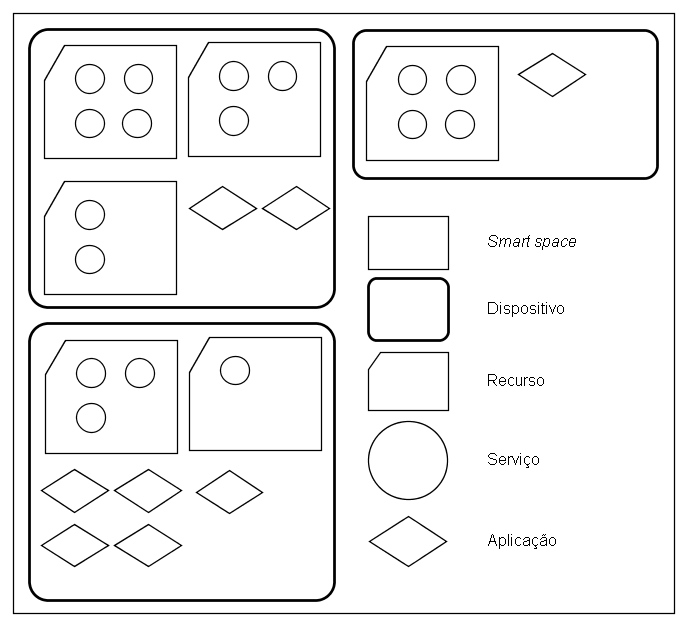
\includegraphics[scale=0.6]{imagens/arquiteturaDSOA}
	\caption{Exemplo da arquitetura DSOA.}
	\label{fig:arquiteturaDSOA}
\end{figure}

Segundo a DSOA, cada recurso, modelado na forma de um \emph{driver}, é identificado por um nome e não há qualquer tipo de relacionamento entre outros recursos. Além disso, o \emph{uOS} não possui uma classificação de recursos. 